This chapter uses the Reference Campaign to establish the behaviour of the frozen nominal model. The analysis begins with the two event-window baselines and then examines the Central Node and geometry responses. Correlation and regression are used only as compact summaries of those responses. The final sections check whether architecture order carries from one event window to the other and show the nominal Pareto trade space. The purpose is to expose the existing performance tensions, not to select a universal optimum from this earlier campaign.

\section{Reference-Campaign Boundary}

The earlier nominal campaign is retained as the historical like-for-like two-event-window architecture sweep. It contains 891 California cases and the same 891 identifiers for India, preserving the baseline comparison under that frozen model. These values are kept separate from Fresh Full891 V2 and are not averaged with the final scenario results in Chapter~7. The contrast is a case-study comparison, not an estimate of a California, India, seasonal, or global population effect.

\section{Validation Status}

All case rows used in this chapter passed the validation procedure in Chapter~5. Specifically, all 1,782 expected case identifiers were present, every case had the expected task population and completed status, and 17,820 independently recomputed metric comparisons agreed with the stored values within $10^{-6}$. Appendix~C records the checks and their evidence. This chapter preserves the Reference Campaign as the frozen nominal baseline. Chapter~7 then presents the unified final Fresh V2 campaign, including the matched regional analysis and the verified 180-satellite evidence.

The analytical population contains 891 cases for California and 891 for India. Every case has the expected task count, and every required case status is completed. Core summary metrics were recomputed from lower-level outputs in 17,820 comparisons with zero failures at a tolerance of $10^{-6}$. The numerical evidence is therefore internally consistent even though external model-validity limitations remain.

\section{Event-Window Campaign Summary}

Table~\ref{tab:regional_summary} gives event-window-normalized means over all 891 architectures. The India workload has the higher mean observation fulfilment, while the California workload reaches a larger share of its useful-recipient set. The mean number of transfer events per task is almost unchanged between the two windows. Data volume per task is higher for California, which contains a larger proportion of the bigger urgent packets.

\begin{table}[htbp]
\centering
\caption{Region-normalized summary across all 891 cases per event region.}
\label{tab:regional_summary}
\begin{tabular}{lrrrrr}
\toprule
Region & Obs. (\%) & \Suseful\ (\%) & Receivers (\%) & Mbit/task & Events/task \\
\midrule
California & 47.47 & 0.62 & 13.87 & 5.88 & 6.19 \\
India & 55.07 & 0.46 & 12.06 & 4.62 & 6.20 \\
\bottomrule
\end{tabular}
\end{table}

The very low mean \Suseful\ values require careful interpretation. They do not mean that almost no task is observed: mean observation fulfilment is roughly 47--55 percent. They mean that completing dissemination to every simulator-defined useful recipient before each deadline is rare under the targeted policy, three-hop limit, and copy limits. Observation requires only one suitably timed observer, while \Suseful\ requires all useful recipients.

\section{Central-Node Fraction Effects}

Figure~\ref{fig:cn_sweep} averages the 81 base geometries at each central-node level. The first step from CN0 to CN10 produces the largest observation gain. Further increases are smaller, and the observation mean falls sharply at CN100. First-reception latency behaves differently: it continues to decrease as the central-node fraction rises. Useful-recipient completion and receiver coverage instead reach their best aggregate values at modest fractions and then decline.

\begin{figure}[htbp]
\centering
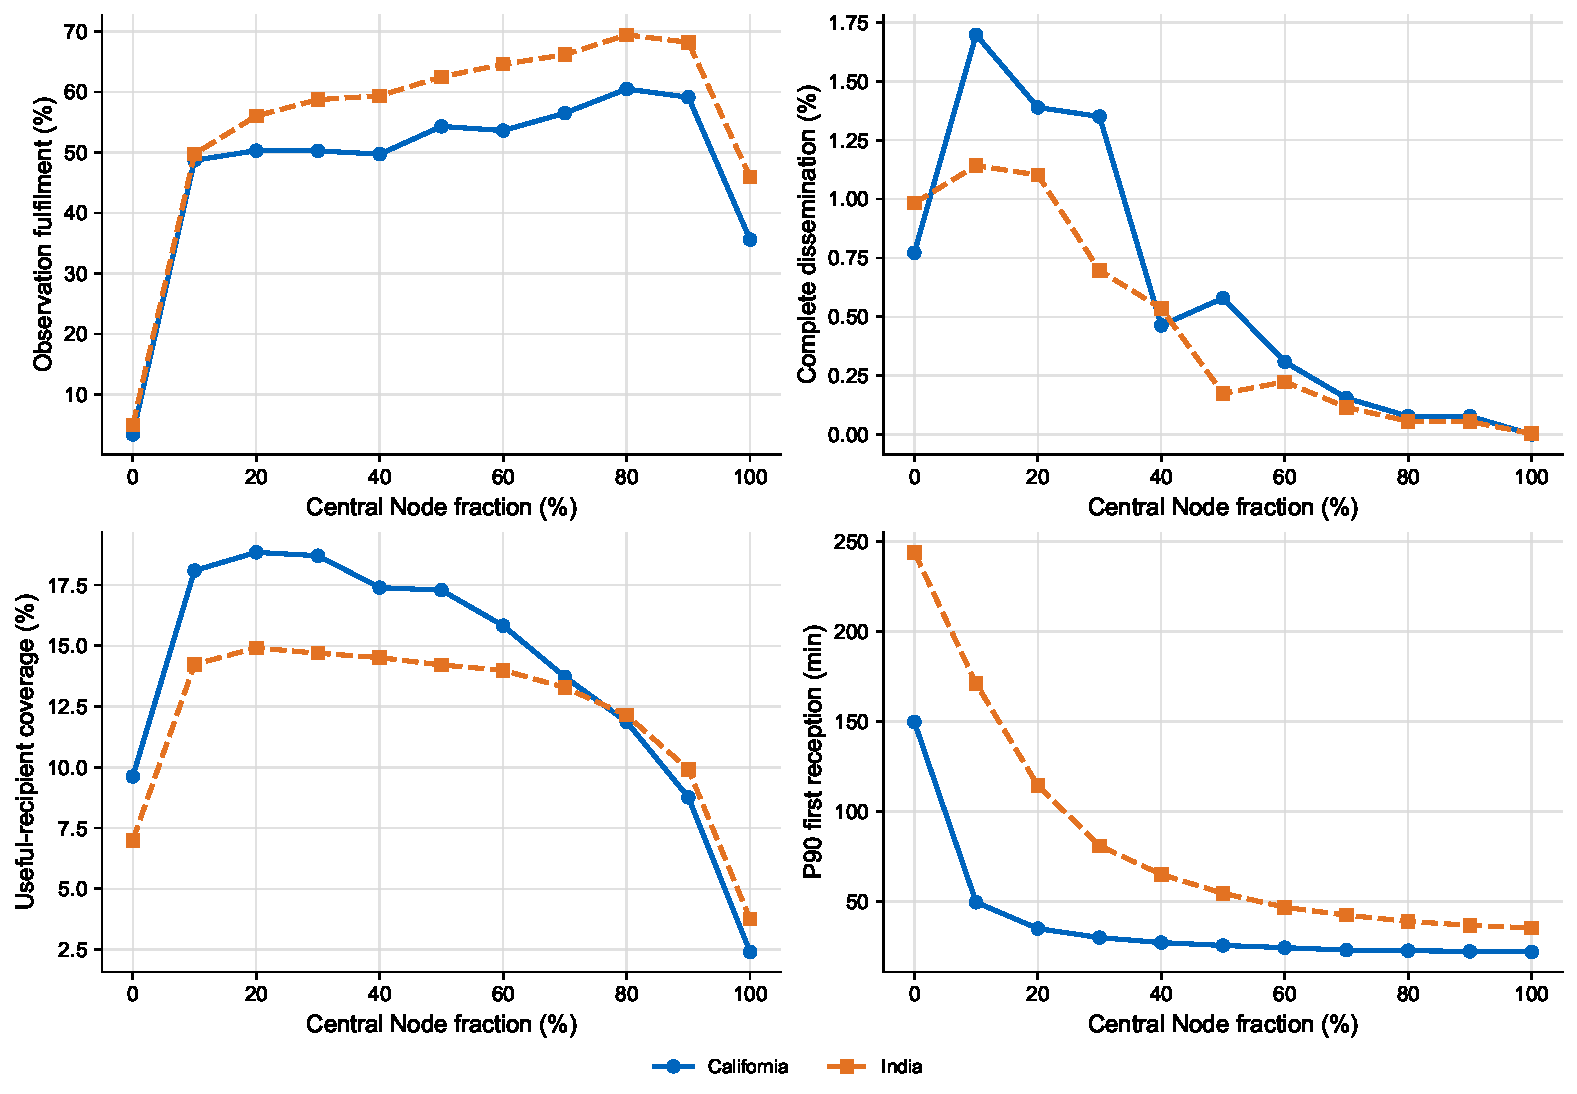
\includegraphics[width=0.98\textwidth]{part2_revision/02_nominal_cn_response.pdf}
\caption{Event-window-specific marginal response to central-node fraction across the full final grid. \Suseful\ denotes complete dissemination to all simulator-defined useful recipients.}
\label{fig:cn_sweep}
\end{figure}

Selected levels are reported in Table~\ref{tab:cn_selected}. The table illustrates the key engineering trade. For California, moving from CN0 to CN10 raises mean observation fulfilment from 3.40 to 48.73 percent and reduces P90 first-reception latency from 149.78 to 49.65 minutes. For India, the corresponding observation change is 4.92 to 49.77 percent and the latency change is 243.94 to 171.06 minutes. Further centralization continues to improve conditional first reception, but useful-recipient breadth does not continue to improve.

\begin{table}[htbp]
\centering
\caption{Selected event-window central-node marginal means across 81 base architectures per row.}
\label{tab:cn_selected}
\begin{tabular}{lrrrrr}
\toprule
Region & CN (\%) & Obs. (\%) & \Suseful\ (\%) & Receivers (\%) & P90 first (min) \\
\midrule
California & 0 & 3.40 & 0.77 & 9.62 & 149.78 \\
California & 10 & 48.73 & 1.70 & 18.10 & 49.65 \\
California & 20 & 50.31 & 1.39 & 18.85 & 35.01 \\
California & 50 & 54.32 & 0.58 & 17.29 & 25.65 \\
California & 80 & 60.49 & 0.08 & 11.87 & 22.77 \\
California & 100 & 35.61 & 0.00 & 2.40 & 22.04 \\
\midrule
India & 0 & 4.92 & 0.98 & 6.99 & 243.94 \\
India & 10 & 49.77 & 1.14 & 14.24 & 171.06 \\
India & 20 & 56.04 & 1.10 & 14.92 & 114.49 \\
India & 50 & 62.50 & 0.17 & 14.21 & 54.63 \\
India & 80 & 69.46 & 0.06 & 12.15 & 38.98 \\
India & 100 & 45.93 & 0.00 & 3.75 & 35.37 \\
\bottomrule
\end{tabular}
\end{table}

\subsection{Observation fulfilment}

The event-window-aggregated observation maximum occurs at 80 percent Central Nodes: 60.49 percent in California and 69.46 percent in India. At 90 percent, both means are slightly lower, and at 100 percent they fall to 35.61 and 45.93 percent. This is the central result of the sweep: the first Central Nodes remove an information bottleneck, but full participation does not preserve that gain under the bounded forwarding package. The decrease is therefore meaningful rather than a cosmetic curve feature, although the bundled treatment does not identify whether forwarding concentration, copy limits, placement, or another package component is responsible.

The highest individual California observation result is 93.75 percent for \path{T060_P05_H0800_I0800_CN050_F1}. The highest India result is 99.09 percent for \path{T180_P10_H1000_I0600_CN090_F1}. Neither of these cases completes \Suseful\ for any task, emphasizing that a case can observe nearly all tasks without disseminating them to every useful recipient.

\subsection{Useful-recipient completion and receiver coverage}

Mean \Suseful\ is small at every aggregate level and reaches its marginal maximum at CN10 in both regions: 1.70 percent for California and 1.14 percent for India. Mean useful-receiver coverage instead peaks at CN20: 18.85 percent for California and 14.92 percent for India. Beyond this point, the number of useful receivers reached by the deadline decreases, particularly at CN100.

The strongest individual \Suseful\ cases are lower-resource 60-satellite configurations. California reaches 25.00 percent for \texttt{T060\_P03\_H0800\_I0986\_CN030\_F1}; India reaches 21.48 percent for \texttt{T060\_P05\_H1000\_I0600\_CN020\_F1}. These same cases also have the largest mean receiver fraction in their region, 47.58 and 45.56 percent, respectively.

The fact that 60-satellite cases dominate this metric is partly mathematical and partly operational. With fewer eligible recipients, completion requires fewer unique arrivals. Larger constellations create more possible observers but also enlarge the dissemination target. This is why \Suseful\ should be compared together with observation fulfilment and resource burden rather than used alone.

\subsection{First-reception latency}

Between CN0 and CN100, conditional P90 first-reception latency falls from 149.78 to 22.04 minutes for California and from 243.94 to 35.36 minutes for India. The shapes are not identical. California obtains most of its reduction by CN20, whereas India continues to improve strongly through CN50. Beyond those levels, each additional reduction is smaller.

The smallest per-case conditional P90 is 1.40 minutes in California and 8.52 minutes in India. These values do not by themselves identify the best architectures. A conditional latency can be small simply because difficult, unfinished tasks have been censored. Any latency comparison must therefore be read together with its completion fraction, which is why the canonical tables retain the censoring columns.

\section{Architecture Factor Effects}

Table~\ref{tab:factor_highlights} collects the most decision-relevant factor-level means. Each entry pools the other factors, so it describes association within the grid rather than a controlled one-factor experiment. The table shows why geometry and centrality cannot be reduced to a single monotonic rule.

\begin{table}[htbp]
\centering
\caption{Selected factor-level marginal effects across the full nominal grid.}
\label{tab:factor_highlights}
\begin{tabularx}{\textwidth}{L{0.16\textwidth}L{0.15\textwidth}Y r r}
\toprule
Region & Factor & Level and interpretation & Mean obs. (\%) & Mean P90 first (min) \\
\midrule
California & Satellites & 60; best mean observation, widest receiver denominator advantage & 51.04 & 44.63 \\
California & Planes & 5; highest observation mean & 55.16 & 27.55 \\
California & Inclination & 60 deg; highest observation and lowest latency & 54.02 & 13.23 \\
California & CN fraction & 80\%; highest mean observation & 60.49 & 22.77 \\
India & Satellites & 120; marginally highest observation mean & 55.57 & 78.79 \\
India & Planes & 10; highest observation mean & 62.27 & 68.98 \\
India & Inclination & 60 deg; strongest regional geometry & 72.42 & 54.22 \\
India & CN fraction & 80\%; highest mean observation & 69.46 & 38.98 \\
\bottomrule
\end{tabularx}
\end{table}

Adding satellites shortens the conditional P90 of first reception, but the fraction of useful receivers reached becomes smaller. Mean receiver coverage falls from 20.95 to 8.55 percent between 60 and 180 satellites in California and from 18.33 to 7.32 percent in India. This does not mean that the larger constellations send fewer messages. Their useful-recipient set grows faster than the bounded-copy policy can cover it.

Plane count affects the two event windows differently. California has its highest mean observation at five planes, while the India workload benefits strongly from ten. Inclination produces the largest event-window contrast: 60 degrees yields 72.42 percent mean observation in India, whereas 98.6 degrees yields 40.43 percent. This is consistent with task latitude and event epoch, but the simulator does not isolate which component is responsible.

Altitude has weaker mean association with observation fulfilment than inclination or plane count. Higher altitude reduces conditional P90 first reception in both regions, but the observation means differ by only a few percentage points across 500, 800, and 1000 km after pooling other factors.

\section{Exploratory Correlation}

Table~\ref{tab:spearman} lists the strongest exploratory rank associations. Higher central-node fraction is associated with lower P90 first-reception latency in both regions. Satellite count is negatively associated with useful-receiver fraction, and inclination shows a strong negative association with India observation fulfilment over the sampled levels.

\begin{table}[htbp]
\centering
\caption{Selected exploratory Spearman associations across 891 cases per region.}
\label{tab:spearman}
\begin{tabularx}{\textwidth}{L{0.17\textwidth}L{0.25\textwidth}Y r}
\toprule
Region & Factor & Metric & $\rho$ \\
\midrule
California & Central Node fraction & P90 first-reception latency & $-0.55$ \\
California & Satellite count & Mean useful-receiver fraction & $-0.56$ \\
California & Plane count & Observation fulfilment & $+0.39$ \\
California & Central Node fraction & Observation fulfilment & $+0.29$ \\
India & Central Node fraction & P90 first-reception latency & $-0.69$ \\
India & Satellite count & Mean useful-receiver fraction & $-0.61$ \\
India & Inclination & Observation fulfilment & $-0.59$ \\
India & Central Node fraction & Observation fulfilment & $+0.34$ \\
\bottomrule
\end{tabularx}
\end{table}

Spearman $\rho$ asks whether the rank of one variable tends to rise or fall with the rank of another; the relation need not be linear. A value close to $+1$ or $-1$ indicates consistent monotonic order, while a value near zero indicates little such order. For India, $\rho=-0.69$ means that higher Central Node fractions are usually associated with lower first-reception latency in this grid. It is not a causal coefficient. Recipient opportunities and all components of the bundled routing treatment change with the fraction, and the calculation pools the remaining architecture factors.

\section{Exploratory Regression of Central-Node Marginal Means}

Figure~\ref{fig:regression_models} compares the best leave-one-level-out model for each event-window response. An exponential-with-offset model describes the steep latency fall better than the polynomial candidates, with leave-one-level-out RMSE of 23.57 minutes for California and 6.29 minutes for India. Quadratic models are preferred for receiver fraction in both event windows, capturing the intermediate peak and later decrease.

\begin{figure}[htbp]
\centering
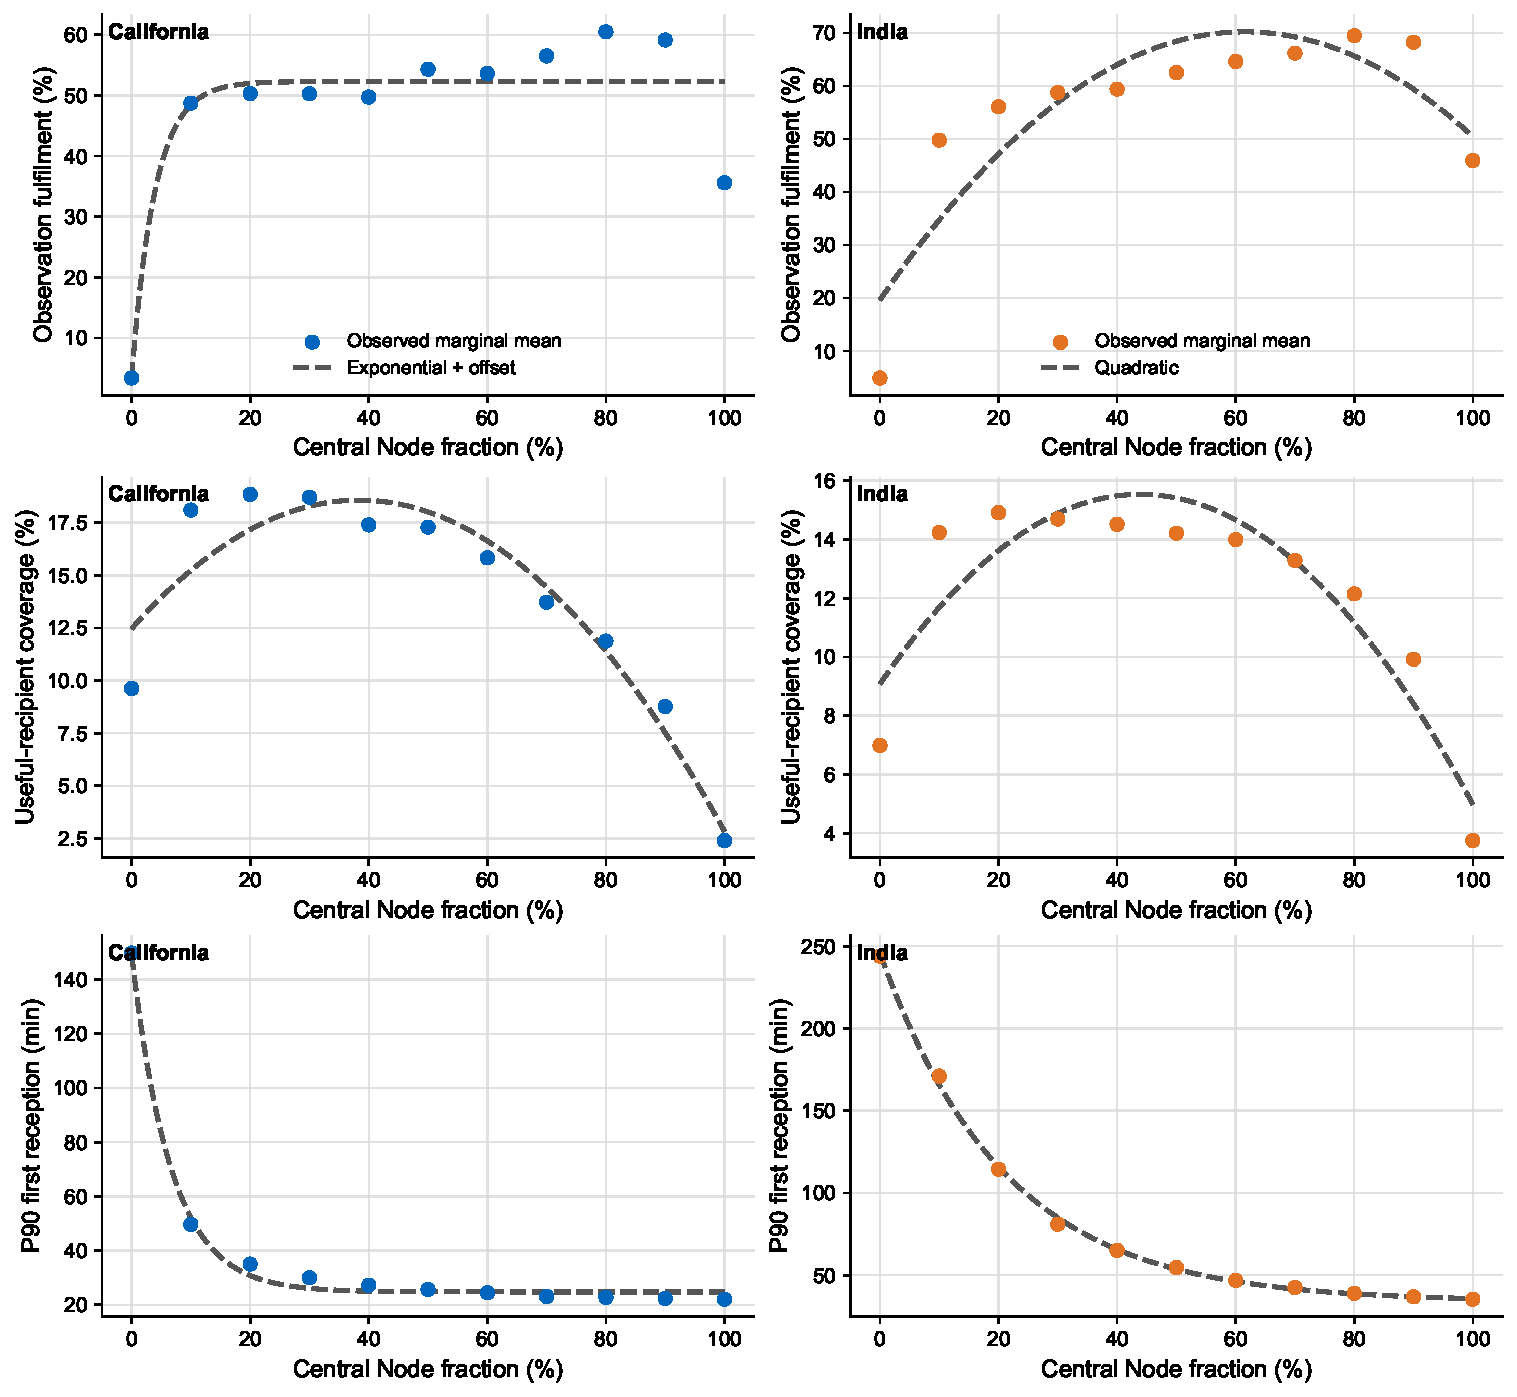
\includegraphics[width=0.98\textwidth]{part2_revision/03_nominal_cn_model_fits.pdf}
\caption{Exploratory regression of the 11 event-window central-node marginal means. The displayed model minimizes leave-one-level-out RMSE among linear, quadratic, cubic, and exponential-with-offset candidates.}
\label{fig:regression_models}
\end{figure}

Table~\ref{tab:regression_best} gives the selected models. California observation has a large cross-validated error despite a high in-sample $R^2$, because a saturating exponential does not reproduce the CN100 decline. This is a warning against treating the fitted curve as a physical law. India observation and both receiver responses are better represented by a quadratic over the sampled range, but extrapolation beyond 0--100 percent is meaningless.

\begin{table}[htbp]
\centering
\caption{Best exploratory regression model by leave-one-central-node-level-out error.}
\label{tab:regression_best}
\begin{tabularx}{\textwidth}{L{0.17\textwidth}Y L{0.25\textwidth}rr}
\toprule
Region & Response & Selected model & $R^2$ & LOOCV RMSE \\
\midrule
California & Observation fulfilment & Exponential + offset & 0.83 & 14.51 \\
California & Useful-receiver fraction & Quadratic & 0.91 & 2.61 \\
California & P90 first reception & Exponential + offset & 1.00 & 23.57 min \\
India & Observation fulfilment & Quadratic & 0.78 & 14.21 \\
India & Useful-receiver fraction & Quadratic & 0.85 & 2.31 \\
India & P90 first reception & Exponential + offset & 1.00 & 6.29 min \\
\bottomrule
\end{tabularx}
\end{table}

The fit statistics are not uniformly ``good''. The latency curves have excellent in-sample $R^2$, but California's 23.57-minute leave-one-level-out error is still operationally large. Observation has lower $R^2$ and approximately 14-percentage-point prediction error because the abrupt CN100 decline is difficult to reconstruct when that level is omitted. Coverage is better behaved, with 2.31--2.61 percentage-point error. Thus the curves summarize saturation and hump-shaped response; they are not reliable laws for interpolation or extrapolation, and they cannot define an optimum without the competing completion and resource objectives.

\section{Paired Event-Window Comparison}

Figure~\ref{fig:regional_paired} places the California and India observation result for each architecture on the same point. The scatter extends well to both sides of the diagonal. Some designs improve for India, others for California, and the ordering cannot be inferred reliably from one event window alone.

\begin{figure}[htbp]
\centering
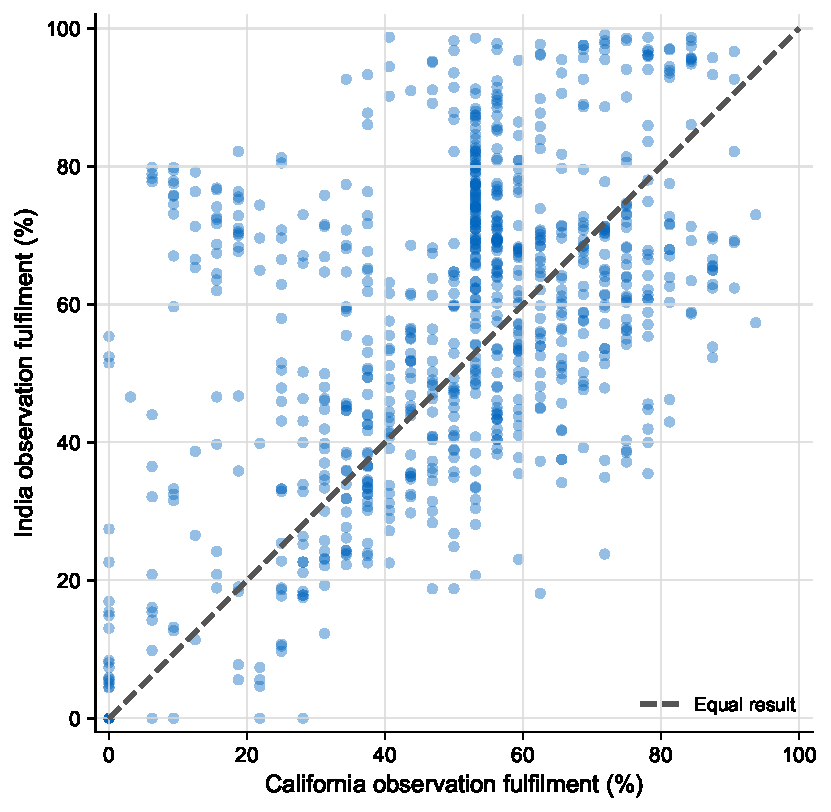
\includegraphics[width=0.72\textwidth]{part2_revision/04_nominal_paired_observation.pdf}
\caption{Paired observation fulfilment for identical architecture identifiers under the California and India task sets.}
\label{fig:regional_paired}
\end{figure}

Rank agreement is reported in Table~\ref{tab:rank_agreement}. A value of 1 would mean that every architecture has the same relative order in both event windows; zero would indicate no monotonic agreement. Conditional P90 first reception and receiver coverage are comparatively stable at 0.78 and 0.74. Observation is only moderately stable at 0.50, and \Suseful\ agreement is 0.11. The last value means that an architecture selected for complete dissemination in one event window provides almost no ranking guarantee in the other. Different task counts, priority mixes, deadlines, and useful-recipient sets therefore alter the decision, not merely the absolute score.

\begin{table}[htbp]
\centering
\caption{Spearman rank agreement between California and India over 891 paired architecture identifiers.}
\label{tab:rank_agreement}
\begin{tabular}{lr}
\toprule
Metric & Rank agreement \\
\midrule
Observation fulfilment & 0.50 \\
\Suseful & 0.11 \\
Mean useful-receiver fraction & 0.74 \\
Conditional P90 first-reception latency & 0.78 \\
\bottomrule
\end{tabular}
\end{table}

\section{Exact Pareto Sets}

Figure~\ref{fig:pareto} plots observation fulfilment against the declared resource-burden proxy and outlines exact Pareto members computed in the full five-objective space. A point can be Pareto optimal even if it appears dominated in this two-dimensional projection, because it may provide better \Suseful, receiver coverage, or conditional latency.

\begin{figure}[htbp]
\centering
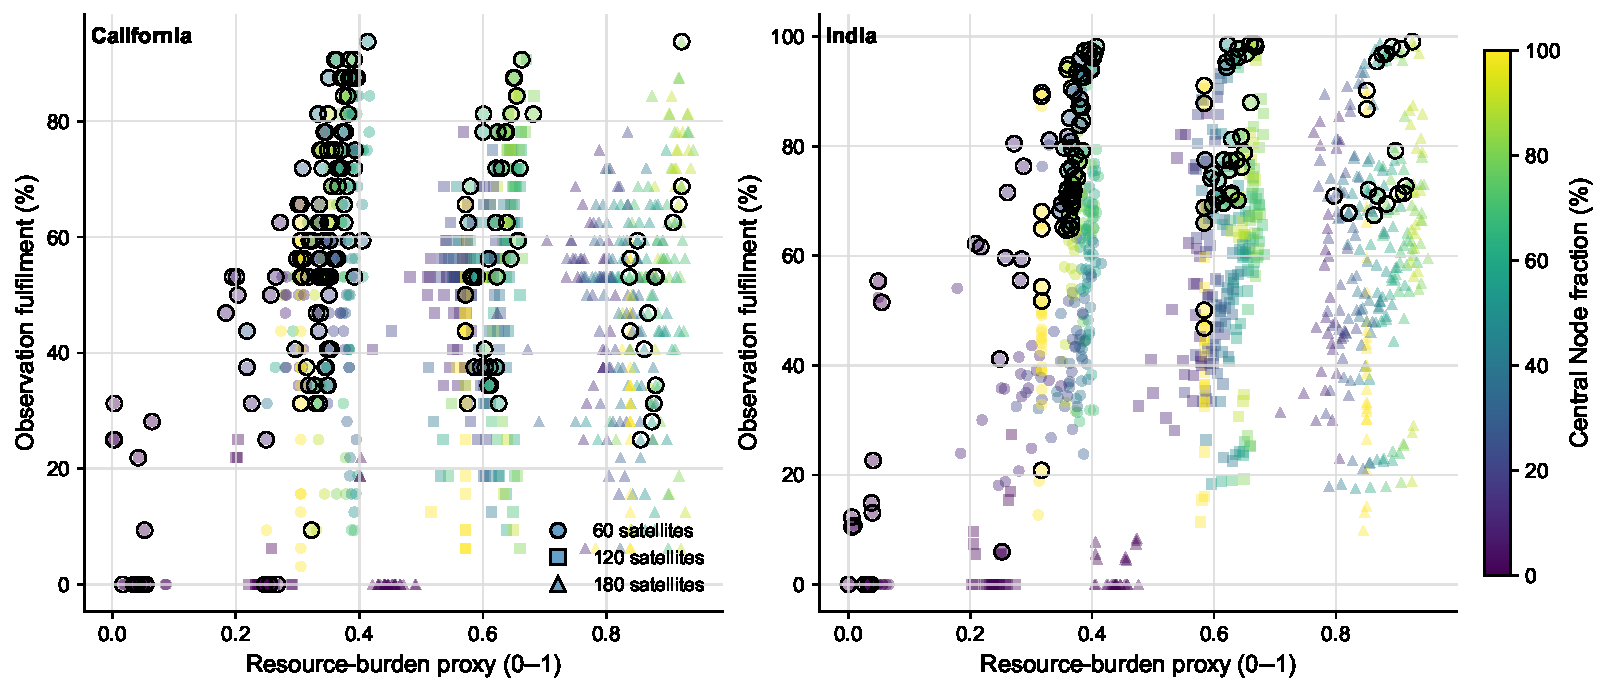
\includegraphics[width=0.98\textwidth]{part2_revision/05_nominal_pareto_landscape.pdf}
\caption{Observation fulfilment versus resource burden, with fleet size shown by marker and Central Node fraction by colour. Black outlines identify cases on the exact five-objective Pareto set.}
\label{fig:pareto}
\end{figure}

The exact fronts contain 183 California cases and 142 India cases, or 20.5 and 15.9 percent of the respective candidate sets. Table~\ref{tab:nominal_pareto_composition} explains which architectures form those fronts. Sixty-satellite cases dominate numerically (125 California and 85 India cases), with a median CN40 configuration. The 180-satellite front is much smaller (17 and 19 cases) and is concentrated at higher Central Node fractions. Smaller fleets therefore survive because they reduce resource burden, whereas larger fleets survive only when their mission benefit compensates for that burden. A single equally weighted score would hide this structure.

\begin{table}[htbp]
\centering
\small
\caption{Composition of the exact nominal Pareto fronts.}
\label{tab:nominal_pareto_composition}
\begin{tabular}{lrrrr}
\toprule
Region & Satellites & Pareto cases & Median CN (\%) & Median observation (\%) \\
\midrule
California & 60 & 125 & 40 & 56.25 \\
California & 120 & 41 & 70 & 56.25 \\
California & 180 & 17 & 80 & 53.13 \\
India & 60 & 85 & 40 & 71.80 \\
India & 120 & 38 & 70 & 77.49 \\
India & 180 & 19 & 70 & 72.70 \\
\bottomrule
\end{tabular}
\end{table}

\section{Nominal Result Synthesis}

The nominal campaign shows a clear separation between early task delivery and broad dissemination. Adding a small central-node population greatly improves observation and first reception relative to CN0 under the central-only topology. Beyond that first step, latency continues to improve, but observation, useful-recipient coverage, and \Suseful\ do not follow a monotonic trend. The bounded copy count and three-hop limit are therefore part of the observed architecture response rather than incidental implementation details.

The paired event-window results add a second constraint: the same architecture does not retain the same rank for California and India. This chapter answers the nominal routing-package and case-study workload questions under the earlier frozen model. It does not establish a population-level regional effect or tolerance to explicit failures; those experiments belong to the Fresh V2 replay in Chapter~7.
